\documentclass[border=10pt]{standalone}
\usepackage{tikz}
\usetikzlibrary{arrows.meta, positioning, fit, backgrounds, calc}
\usepackage[T1]{fontenc}
\usepackage{helvet}
\renewcommand{\familydefault}{\sfdefault}

\definecolor{darkblue}{RGB}{0, 0, 139}
\definecolor{pinkdash}{RGB}{255, 50, 120}

\begin{document}
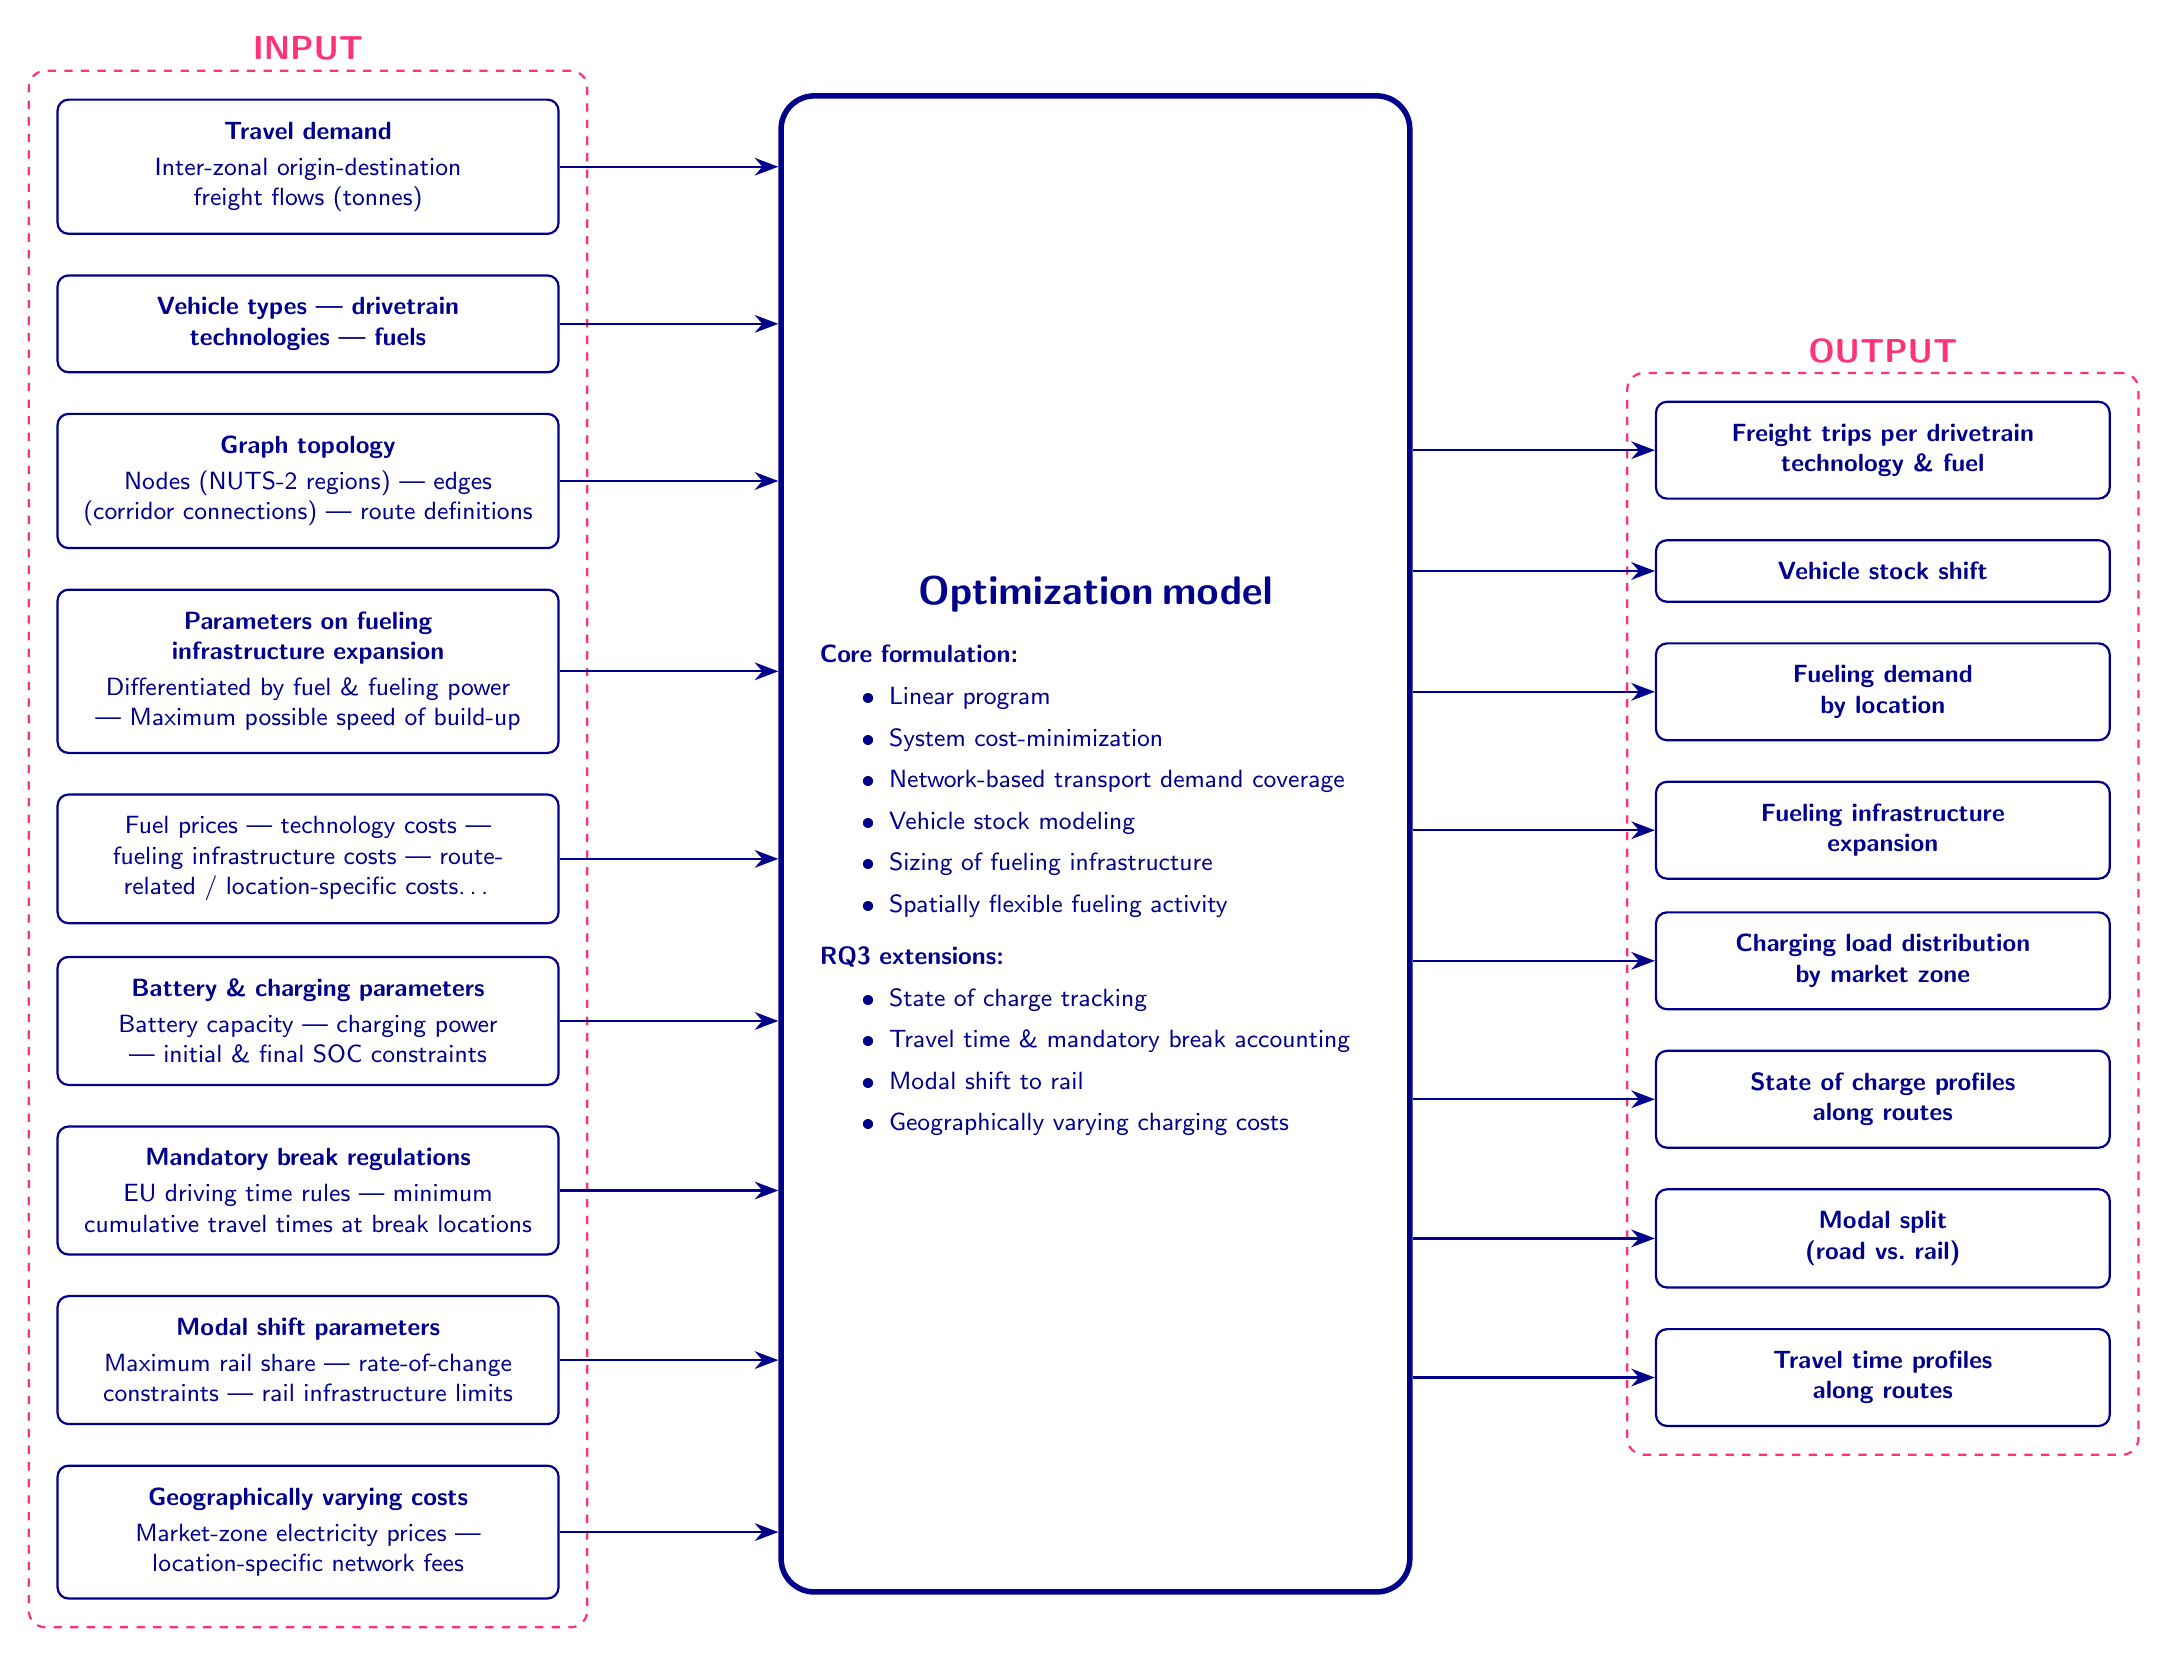
\begin{tikzpicture}[
    node distance=0.5cm,
    inputbox/.style={
        draw=darkblue, thick, rounded corners=4pt,
        text width=5.8cm, align=center, inner sep=8pt,
        font=\small, text=darkblue
    },
    outputbox/.style={
        draw=darkblue, thick, rounded corners=4pt,
        text width=5.2cm, align=center, inner sep=8pt,
        font=\small\bfseries, text=darkblue
    },
    modelbox/.style={
        draw=darkblue, line width=2pt, rounded corners=12pt,
        text width=7cm, align=left, inner sep=14pt,
        font=\small, text=darkblue
    },
    arrow/.style={-{Stealth[length=3mm]}, darkblue, thick},
    dashed border/.style={draw=pinkdash, dashed, thick, rounded corners=6pt}
]

% MODEL BOX - placed first as the central anchor
\node[modelbox, minimum height=19cm] at (10, -10) (model) {
    \begin{center}\textbf{\Large Optimization model}\end{center}\vspace{2pt}
    \textbf{Core formulation:}
    \begin{itemize}
        \setlength{\itemsep}{2pt}
        \item Linear program
        \item System cost-minimization
        \item Network-based transport demand coverage
        \item Vehicle stock modeling
        \item Sizing of fueling infrastructure
        \item Spatially flexible fueling activity
    \end{itemize}
    \vspace{4pt}
    \textbf{RQ3 extensions:}
    \begin{itemize}
        \setlength{\itemsep}{2pt}
        \item State of charge tracking
        \item Travel time \& mandatory break accounting
        \item Modal shift to rail
        \item Geographically varying charging costs
    \end{itemize}
};

% INPUT BOXES - vertically centered on the lower half of the model box
\node[inputbox] at (0, -1.4) (input1) {
    \textbf{Travel demand}\\[2pt]
    Inter-zonal origin-destination freight flows (tonnes)
};

\node[inputbox, below=of input1] (input2) {
    \textbf{Vehicle types | drivetrain\\technologies | fuels}
};

\node[inputbox, below=of input2] (input3) {
    \textbf{Graph topology}\\[2pt]
    Nodes (NUTS-2 regions) | edges (corridor connections) | route definitions
};

\node[inputbox, below=of input3] (input4) {
    \textbf{Parameters on fueling\\infrastructure expansion}\\[2pt]
    Differentiated by fuel \& fueling power | Maximum possible speed of build-up
};

\node[inputbox, below=of input4] (input5) {
    Fuel prices | technology costs | fueling infrastructure costs | route-related / location-specific costs\ldots
};

% ADDITIONAL RQ3 INPUTS
\node[inputbox, below=0.4cm of input5] (input6) {
    \textbf{Battery \& charging parameters}\\[2pt]
    Battery capacity | charging power | initial \& final SOC constraints
};

\node[inputbox, below=of input6] (input7) {
    \textbf{Mandatory break regulations}\\[2pt]
    EU driving time rules | minimum cumulative travel times at break locations
};

\node[inputbox, below=of input7] (input8) {
    \textbf{Modal shift parameters}\\[2pt]
    Maximum rail share | rate-of-change constraints | rail infrastructure limits
};

\node[inputbox, below=of input8] (input9) {
    \textbf{Geographically varying costs}\\[2pt]
    Market-zone electricity prices | location-specific network fees
};

% OUTPUT BOXES - core outputs placed in upper portion
\node[outputbox] at (20, -5) (output1) {
    Freight trips per drivetrain\\technology \& fuel
};

\node[outputbox, below=of output1] (output2) {
    Vehicle stock shift
};

\node[outputbox, below=of output2] (output3) {
    Fueling demand\\by location
};

\node[outputbox, below=of output3] (output4) {
    Fueling infrastructure\\expansion
};

% ADDITIONAL RQ3 OUTPUTS
\node[outputbox, below=0.4cm of output4] (output5) {
    Charging load distribution\\by market zone
};

\node[outputbox, below=of output5] (output6) {
    State of charge profiles\\along routes
};

\node[outputbox, below=of output6] (output7) {
    Modal split\\(road vs.\ rail)
};

\node[outputbox, below=of output7] (output8) {
    Travel time profiles\\along routes
};

% ARROWS: INPUT -> MODEL
\draw[arrow] (input1.east) -- (input1.east -| model.west);
\draw[arrow] (input2.east) -- (input2.east -| model.west);
\draw[arrow] (input3.east) -- (input3.east -| model.west);
\draw[arrow] (input4.east) -- (input4.east -| model.west);
\draw[arrow] (input5.east) -- (input5.east -| model.west);
\draw[arrow] (input6.east) -- (input6.east -| model.west);
\draw[arrow] (input7.east) -- (input7.east -| model.west);
\draw[arrow] (input8.east) -- (input8.east -| model.west);
\draw[arrow] (input9.east) -- (input9.east -| model.west);

% ARROWS: MODEL -> OUTPUT
\draw[arrow] (model.east |- output1.west) -- (output1.west);
\draw[arrow] (model.east |- output2.west) -- (output2.west);
\draw[arrow] (model.east |- output3.west) -- (output3.west);
\draw[arrow] (model.east |- output4.west) -- (output4.west);
\draw[arrow] (model.east |- output5.west) -- (output5.west);
\draw[arrow] (model.east |- output6.west) -- (output6.west);
\draw[arrow] (model.east |- output7.west) -- (output7.west);
\draw[arrow] (model.east |- output8.west) -- (output8.west);

% DASHED BORDERS
\begin{scope}[on background layer]
    \node[dashed border, fit=(input1)(input9), inner sep=10pt, label={[text=pinkdash, font=\bfseries\large]above:INPUT}] {};
    \node[dashed border, fit=(output1)(output8), inner sep=10pt, label={[text=pinkdash, font=\bfseries\large]above:OUTPUT}] {};
\end{scope}

\end{tikzpicture}
\end{document}
